\chapter{Introduction}

\section{Background and motivation}


Numerical simulations have become an indispensable tool across numerous domains of engineering and applied sciences, significantly impacting design, analysis, and optimization processes. Their use spans many areas: from the structural design of complex infrastructures \cite{carrera2014finite, ranzi2018structural}, advanced vehicle development \cite{stork2008towards}, to the modeling of intricate natural phenomena \cite{gingold1977smoothed}, and the optimization of industrial operations \cite{kiran2020numerical,davidson2003role}. By leveraging simulation-based approaches, researchers and engineers can explore, predict, and optimize the behavior of physical systems efficiently, significantly reducing dependence on costly, time-consuming, and potentially hazardous experimental campaigns \cite{belytschko2014nonlinear,zienkiewicz2005finite}.

The widespread adoption and success of simulation methods have been propelled by substantial advances in computational power, algorithmic accuracy, and the growing availability of high-resolution datasets \cite{Gunal2019Industry, Rodic2017Industry}. In recent years, these advancements have paved the way for transformative technological paradigms such as Industry 4.0 and, more recently, Industry 5.0. These paradigms integrate advanced simulations with real-time sensor data and artificial intelligence, fostering cyber-physical systems that exhibit greater autonomy, adaptability, and operational efficiency \cite{Agostino2020Using, Onggo2018SYMBIOTIC, Catelani2021From}. Within these evolving frameworks, high-fidelity simulations provide critical support for real-time decision-making, predictive analytics, and the design of intelligent manufacturing and monitoring systems \cite{Sandberg2019Current, Muhammet2021Industry, Muhuri2019Industry}.

Nevertheless, as model fidelity and complexity escalate, computational demands have grown considerably \cite{elmisaoui2023high}. High-resolution simulations, essential for accurately capturing intricate physical behaviors, often necessitate extensive computational resources and prolonged execution times on high-performance computing (HPC) infrastructures \cite{hosseini2016direct}. This computational intensity significantly limits their practical deployment in scenarios demanding rapid response, including real-time control \cite{ra2023real, ballin1988high}, extensive parametric optimization studies \cite{breitkopf2013multidisciplinary}, and continuous monitoring of dynamic systems \cite{dyskin2018computational}.

To overcome these limitations, the development and adoption of reduced order models (ROMs) have gained prominence. ROMs efficiently encapsulate the essential dynamics of complex systems within reduced-dimensional representations, achieving substantial reductions in computational cost while preserving the accuracy of the underlying high-fidelity models \cite{quarteroni2015reduced}. Integrating these ROMs with modern machine learning approaches has further enhanced their ability to effectively capture nonlinear behaviors, improve model generalization, and broaden applicability across varying operational conditions \cite{lee2020model}.

Furthermore, embedding ROMs within comprehensive operational frameworks, particularly digital twins, has opened new horizons for real-time simulation-based optimization and continuous system monitoring \cite{kapteyn2022data}. Digital twins, empowered by ROMs and machine learning, enable precise, dynamic, and actionable insights into physical systems, representing a powerful synthesis of simulation, data-driven modeling, and real-time analytics.

In this context, the research presented herein aims to advance the development and integration of ROM methodologies and machine learning techniques. The goal is to effectively address contemporary computational challenges, fostering more responsive, accurate, and cost-effective simulation solutions tailored to the rigorous demands of modern engineering and industrial applications.

Several European research initiatives provide a direct backdrop to these objectives. For instance, the \href{https://cordis.europa.eu/project/id/800898}{ExaQUte} project~\cite{tosi2021parallel} laid the theoretical and computational groundwork for scalable exascale simulations, particularly in uncertainty quantification (UQ) and optimization under uncertainty. In parallel, the \href{https://cordis.europa.eu/project/id/946009}{EdgeTwins} project extended these exascale-driven insights into real-time digital twins running on constrained devices, demonstrating the viability of linear ROMs in edge deployments. Building on both, the \href{https://www.eflows4hpc.eu/}{eFlows4HPC} project~\cite{ejarque2022enabling} offers a unified workflow framework that integrates HPC, data analytics, and artificial intelligence for large-scale digital twin deployment (see Figure~\ref{fig:rom_workflow_eflows}). Within these efforts, ROMs serve as the linchpin for bridging high-fidelity physics with the fast, adaptive, and resource-efficient requirements of modern cyber-physical systems.

\begin{figure}[ht]
    \centering
    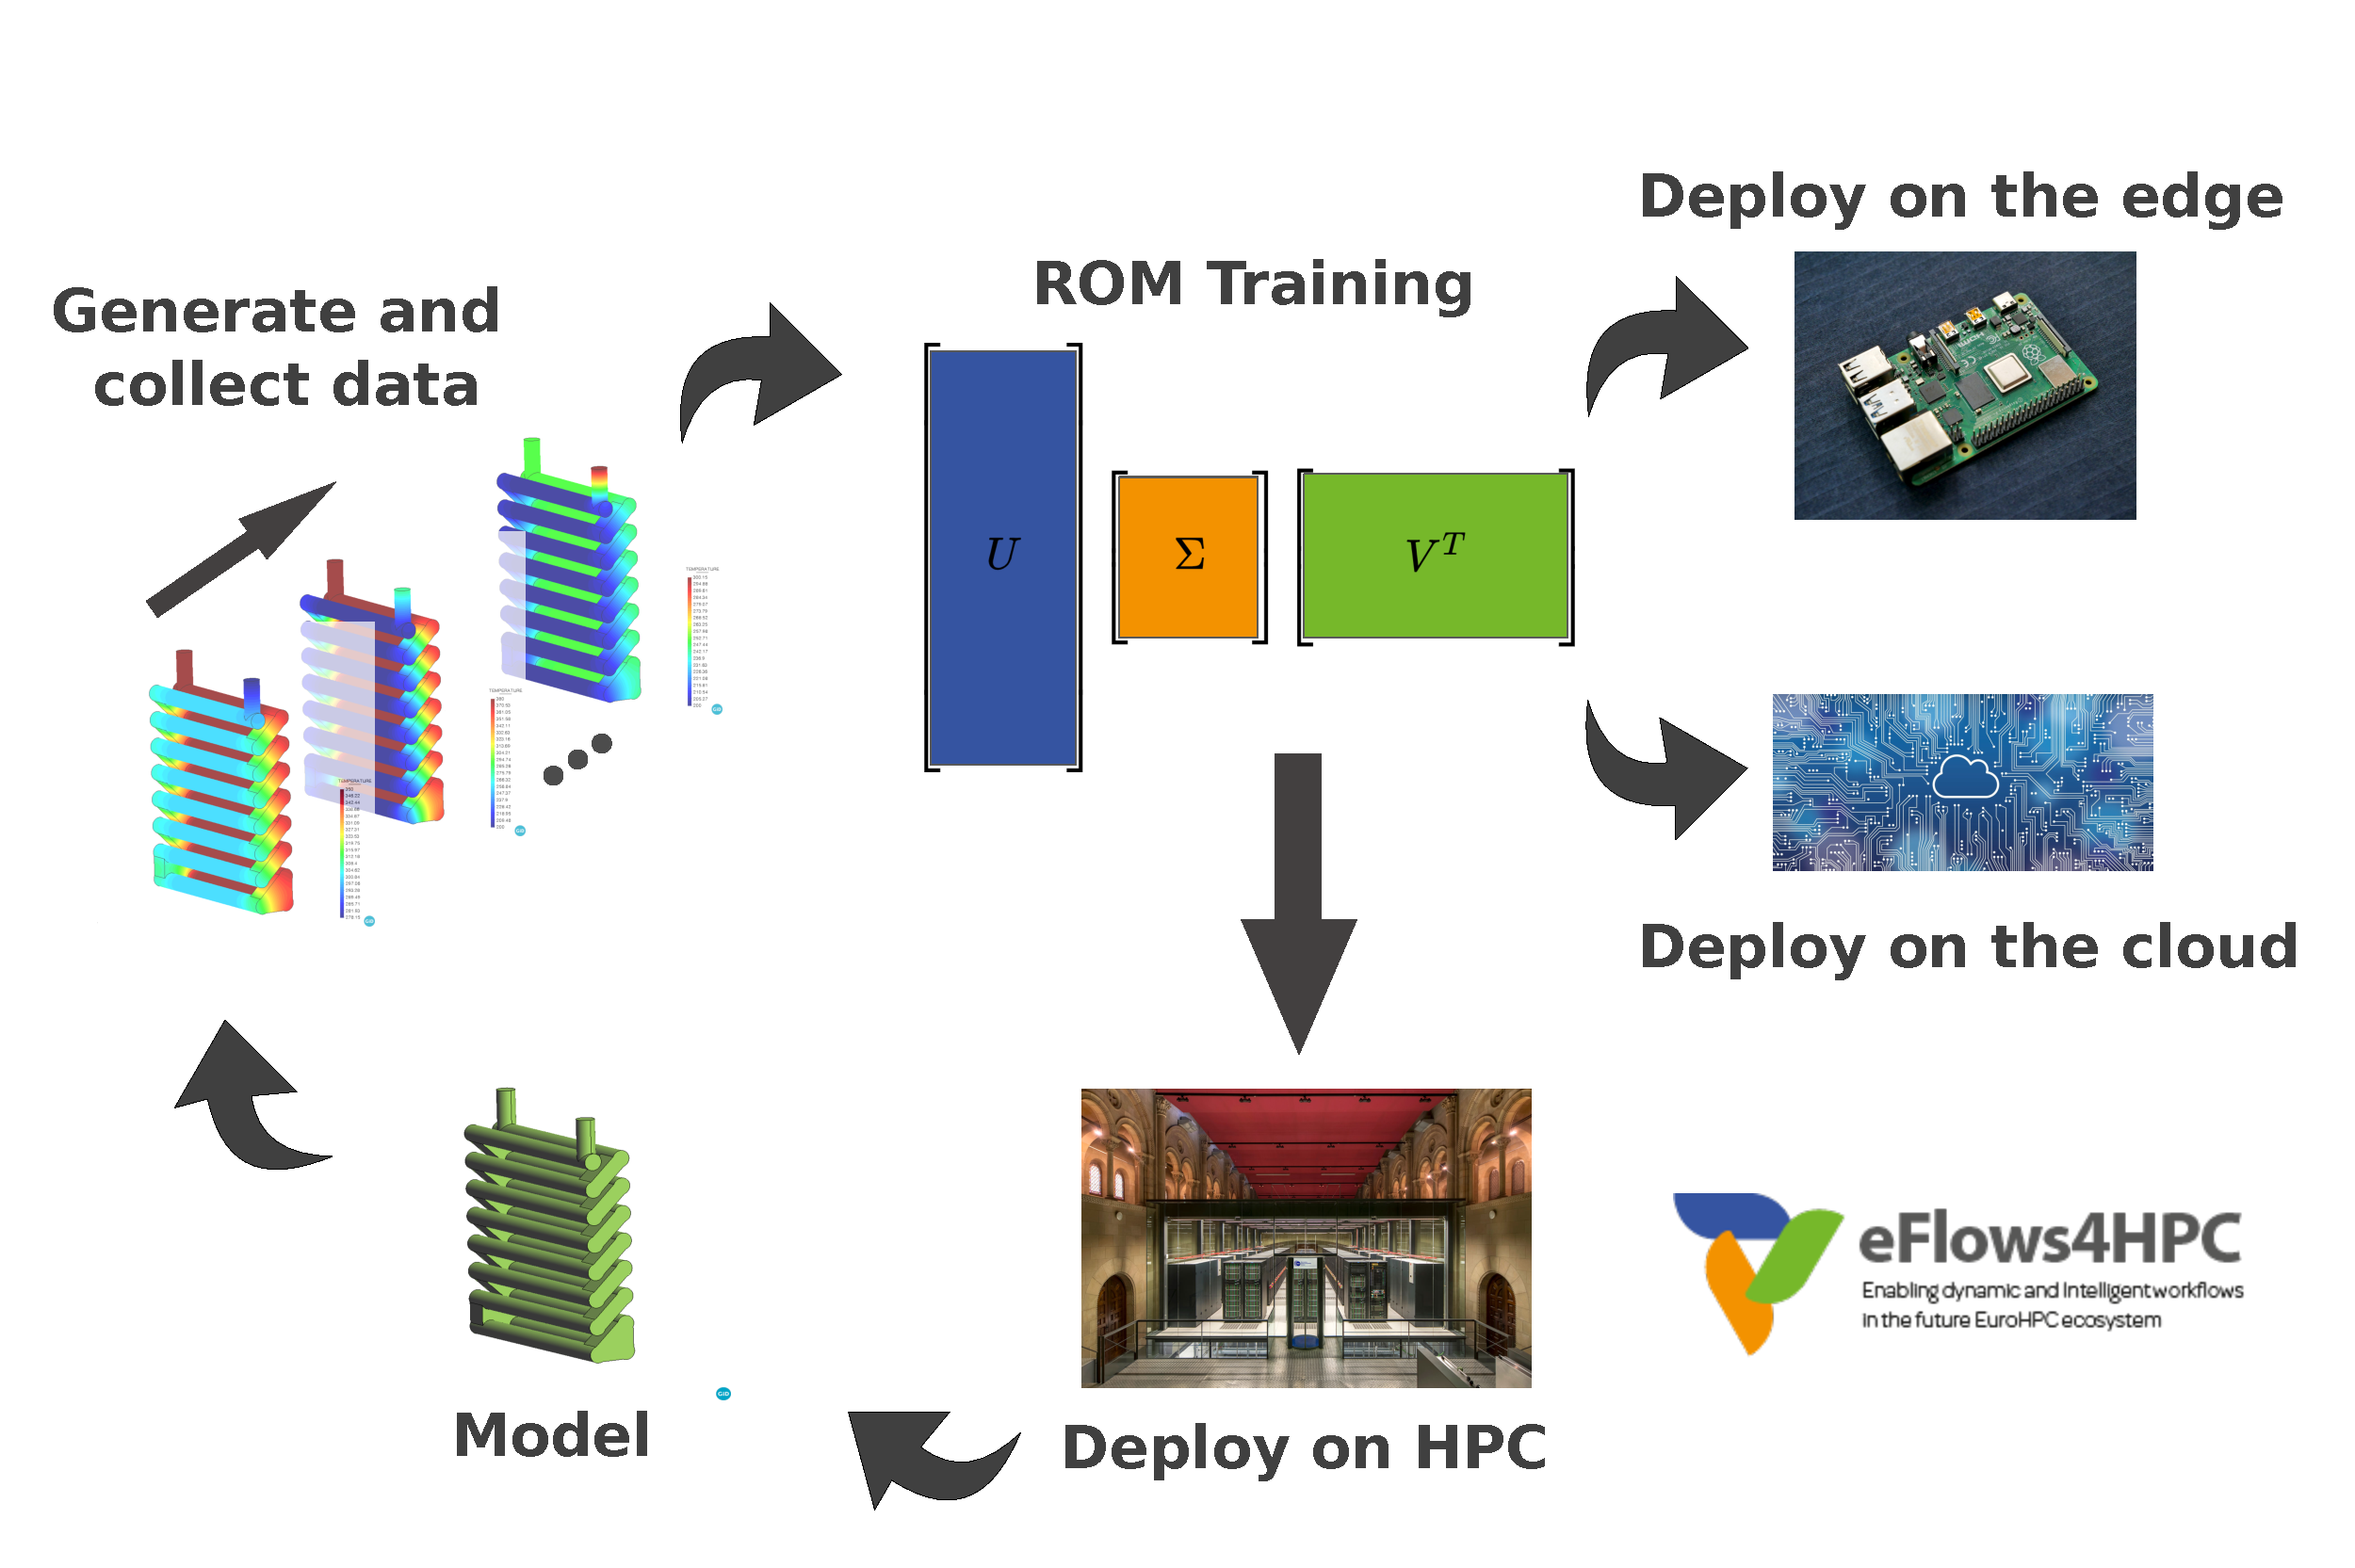
\includegraphics[width=0.92\textwidth]{Figures/Poster.pdf}
    \caption{Main phases in the ROM workflow: data generation using high-fidelity simulations, training via dimensionality reduction, and deployment on target platforms (cloud, edge, HPC). Adapted from~\cite{ejarque2022enabling}.}
    \label{fig:rom_workflow_eflows}
\end{figure}


By leveraging this broader ecosystem of HPC-enabled simulation, reduced order modeling, and digital twin technologies, the present thesis consolidates and extends these efforts through four core research directions:

(1) the development of hyper-reduction techniques for Petrov–Galerkin projection-based ROMs, enabling efficient acceleration for convection-dominated systems~\cite{Ares2023};

(2) the design of scalable, parallel workflows for the training and deployment of projection-based reduced order models on HPC infrastructures, enabling real-time digital twin applications~\cite{Ares2024};

(3) the introduction of a discrete physics-informed training strategy for projection-based ROMs, ensuring that learned nonlinear manifolds remain consistent with the governing residual structure during intrusive projection~\cite{sibuet2025discrete};

and (4) the extension and systematic assessment of nonlinear closure strategies based on machine learning, specifically, radial basis functions (RBF) and Gaussian processes (GP), to improve robustness and interpretability for strongly nonlinear problems~\cite{de2025nonlinear}.

Together, these contributions address key computational bottlenecks and advance the state-of-the-art and practical deployment of projection-based ROMs in high-dimensional, real-time industrial digital twin applications.



\section{Literature review}
\subsection{High-fidelity modeling: Numerical methods in engineering}

High-fidelity numerical simulations are essential tools for understanding, predicting, and optimizing complex physical phenomena in engineering. These simulations are generally based on mathematical models expressed as partial differential equations (PDEs), which describe diverse physical behaviors across numerous disciplines. Due to the inherent complexity of solving PDEs analytically, numerical methods have become indispensable for practical engineering solutions.

Among the most established and versatile numerical approaches are the Finite Element Method (FEM), particularly effective for structural mechanics, fluid-structure interaction, and multiphysics simulations \cite{zienkiewicz2005finite,onate2009structural}; the Finite Difference Method (FD), widely used for wave propagation, heat conduction, and electromagnetics due to its simplicity and ease of implementation \cite{mitchell1980finite,taflove2005computational}; and the Finite Volume Method (FV), favored for fluid dynamics applications owing to its robust enforcement of conservation principles across control volumes \cite{versteeg2007introduction,moukalled2016finite}. Throughout this thesis and its associated publications, these three methodologies constitute the core numerical strategies employed.

Each of these high-fidelity numerical methods has achieved remarkable maturity, integrating advanced discretization techniques, adaptive meshing, and multiphysics coupling. However, their high accuracy comes at significant computational costs, demanding extensive computational resources and specialized hardware, particularly problematic in real-time, optimization-driven, or resource-constrained scenarios. These limitations motivate the pursuit of faster, more efficient surrogate models that can emulate high-fidelity simulations at a fraction of the cost, particularly ROMs, which offer a promising trade-off between accuracy and computational efficiency. The ROMs developed and analyzed in this thesis are consistently formulated using a discrete residual framework, ensuring seamless integration across FEM, FD, and FV schemes. These models are implemented using a combination of open-source and in-house simulation tools, including 
\href{https://github.com/KratosMultiphysics/Kratos}{Kratos Multiphysics}~\cite{dadvand2010object}, 
\href{https://bitbucket.org/frg/aero-f/src/master/}{AERO-F}, 
and academic solvers developed in Python and C++.



\subsection{Reduced order modeling}

The high computational cost associated with high-fidelity numerical simulations has motivated the development of surrogate modeling strategies capable of accelerating repeated or real-time evaluations. In many applications, including parametric studies, optimization loops, uncertainty quantification, and digital twins, traditional solvers become impractical due to their high dimensionality and intensive resource demands~\cite{brunton2022data, rozza2022advanced}.

ROMs offer a powerful alternative by seeking low-dimensional representations that approximate the behavior of complex systems with significantly reduced computational effort. The central assumption behind ROMs is that, despite the high dimensionality of the full-order model (FOM), the set of solutions of interest often lies on or near a low-dimensional manifold embedded in the high-dimensional space~\cite{ryckelynck2024manifold}.

Among the most widely used ROM techniques are those based on linear dimensionality reduction. The Proper Orthogonal Decomposition (POD) is one of the most established methods and extracts dominant modes from a set of solution snapshots (see Figure~\ref{fig:pod_snapshots_overview}) using techniques such as singular value decomposition (SVD), which provides a compressed, low-rank approximation of the snapshot matrix by extracting a reduced basis from its dominant patterns (see Figure~\ref{fig:svd_illustration})~\cite{Sirovich1987, Balachandar1998}.
Other classical approaches include the Reduced Basis (RB) method~\cite{hesthaven2016certified, hesthaven2022reduced}, which constructs reduced spaces tailored to parametric PDEs, and the Proper Generalized Decomposition (PGD)~\cite{nouy2010priori}, which decomposes multivariate functions into separable representations.

\begin{figure}[htbp!]
    \centering
    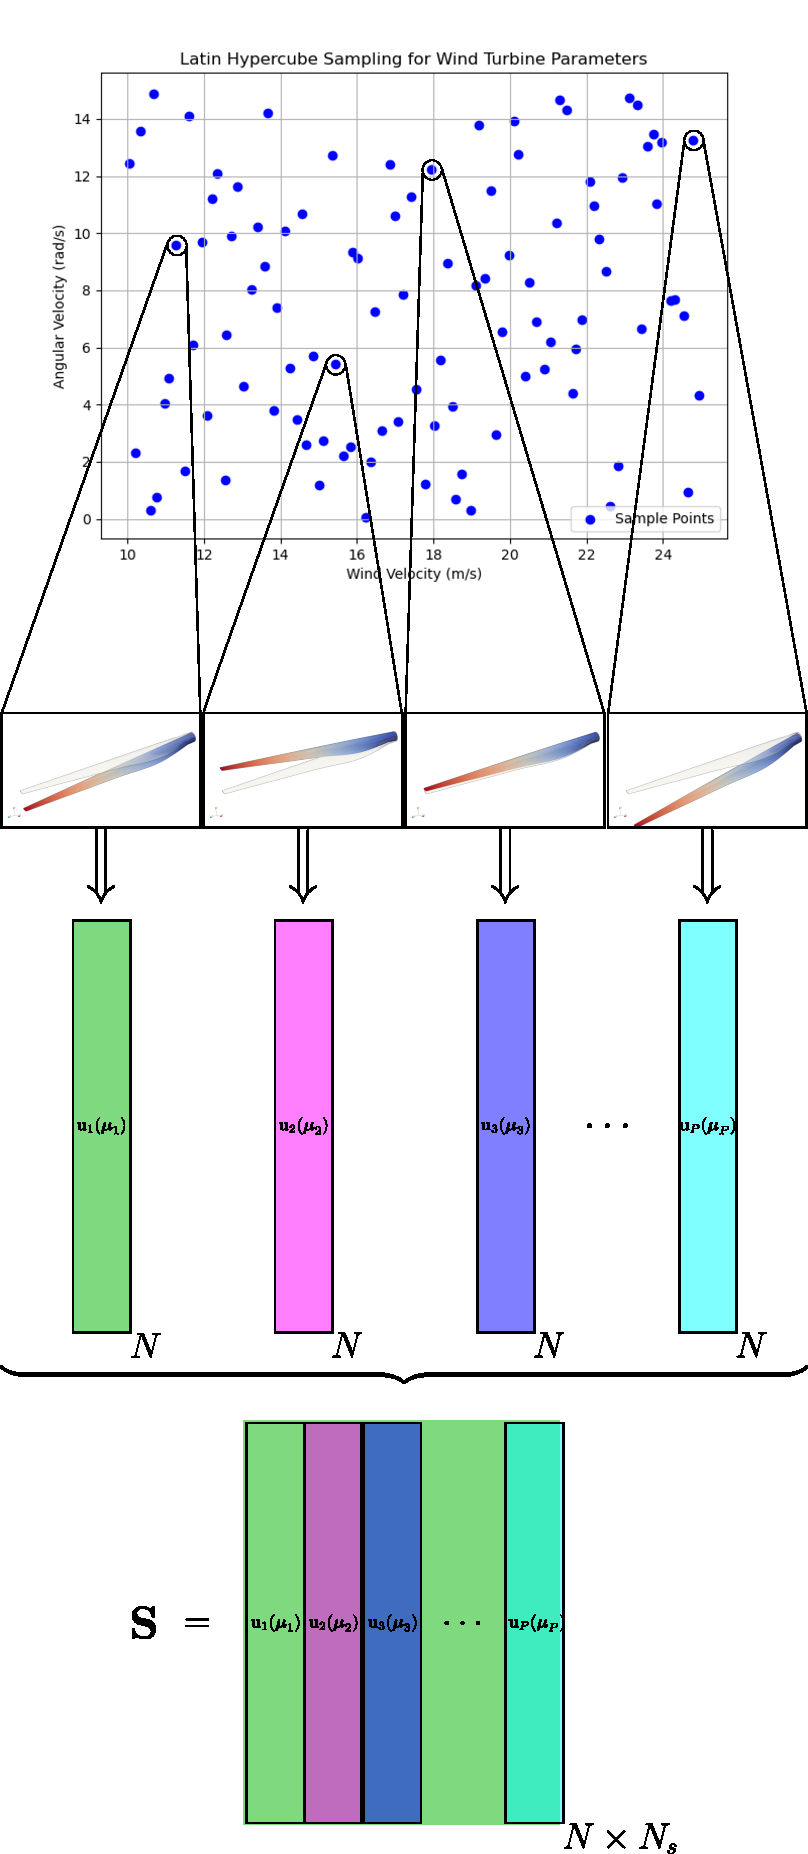
\includegraphics[width=0.5\textwidth]{Figures/SnapshotMatrixConstruction.pdf}
    \caption{Illustration of snapshot matrix construction for a structural model of a wind turbine blade. A set of training points, here defined by angular velocity and wind speed (sampled via Latin Hypercube Sampling), leads to parallel high-fidelity simulations whose results are stored in vectors and stacked to form the snapshot matrix~$\mathbf{S}$.}
    \label{fig:pod_snapshots_overview}
\end{figure}

\begin{figure}[htbp!]
    \centering
    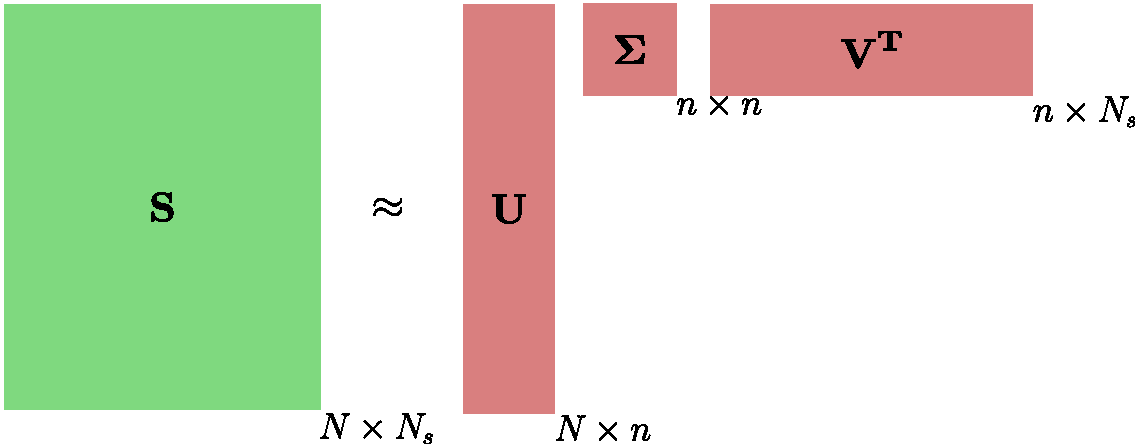
\includegraphics[width=0.7\textwidth]{Figures/SVD_Decomposition.pdf}
    \caption{Visual interpretation of the Singular Value Decomposition. The high-dimensional snapshot matrix~$\mathbf{S}$ is approximately factorized into a reduced basis~$\mathbf{U}$, a diagonal matrix of singular values~$\boldsymbol{\Sigma}$, and temporal or parametric coefficients~$\mathbf{V^T}$. This structure allows for compression and efficient low-dimensional representation.}
    \label{fig:svd_illustration}
\end{figure}



A robust strategy for constructing ROMs, known as projection-based reduced order models (PROMs), involves projecting the governing equations of the full-order model onto a reduced space spanned by the dominant modes (see Figure~\ref{fig:galerkin_prom_visual}). These PROMs rely on the assumption that the system dynamics can be accurately represented in a lower-dimensional subspace derived from high-fidelity snapshots. In the classical Galerkin projection, the residual of the governing equations is enforced to be orthogonal to the reduced basis, making it particularly effective for problems with symmetric positive definite (SPD) operators~\cite{carlberg2017galerkin, benner2015survey, Rowley2004}. For more general problems, especially those dominated by convection or exhibiting non-symmetric Jacobians, the Least-Squares Petrov–Galerkin (LSPG) approach offers a more robust alternative by minimizing the discrete residual in a least-squares sense~\cite{carlberg2011efficient}. While LSPG has proven effective in finite difference and finite volume contexts, its implementation in finite element settings often requires auxiliary constructions to enable efficient approximation. In this thesis, we explore an alternative yet equivalent Petrov–Galerkin formulation tailored for finite element discretizations, specifically designed to preserve element-level assembly during least-squares residual minimization. This modification anticipates the challenges posed by hyper-reduction in nonlinear settings and enables seamless integration of PROMs with efficient mesh-based approximation strategies~\cite{Ares2023}.

\begin{figure}[ht]
    \centering
    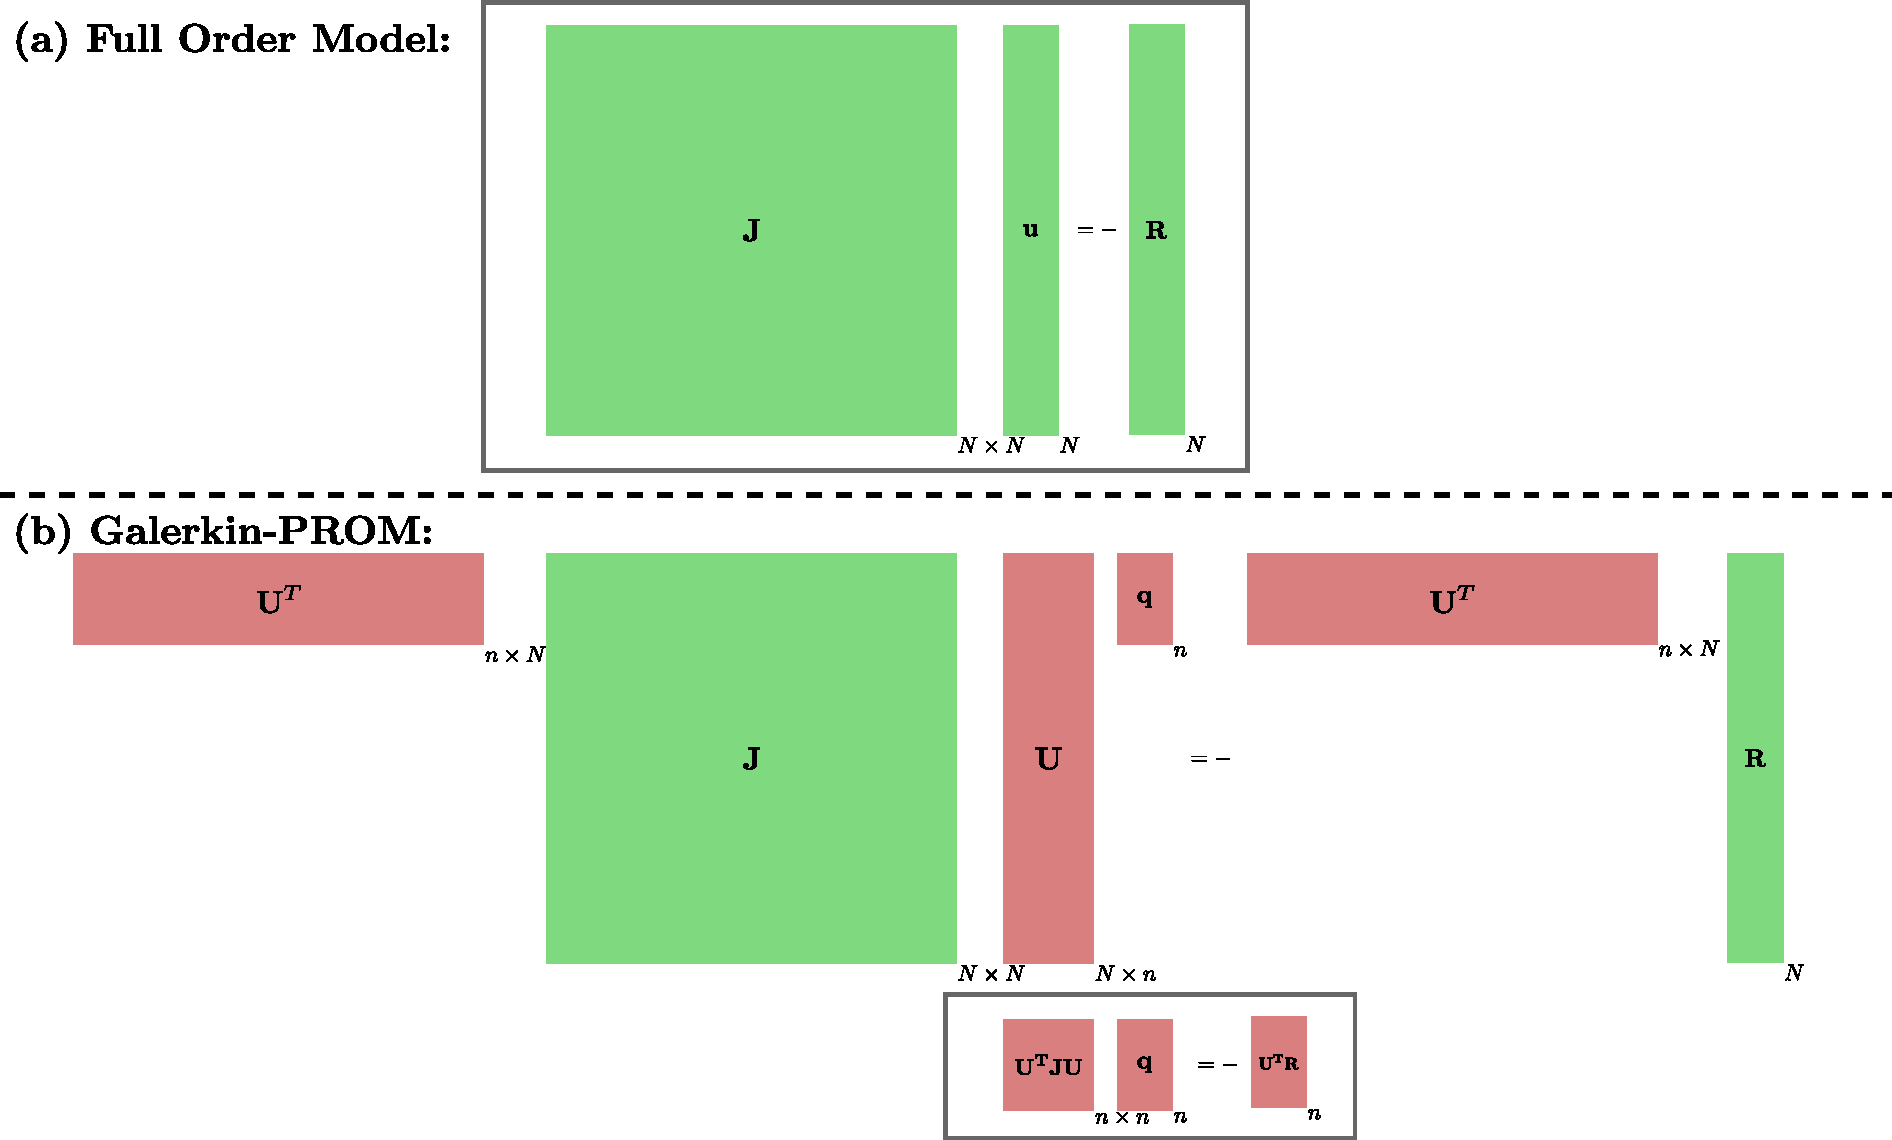
\includegraphics[width=0.95\textwidth]{Figures/SystemReduction.pdf}
    \caption{Schematic comparison between the full-order model and its Galerkin projection-based reduced order model. The full system of dimension~$N$ is projected onto a reduced space of dimension~$n$ using a basis~$\mathbf{U}$, yielding a smaller system with the same governing structure but much lower computational cost.}
    \label{fig:galerkin_prom_visual}
\end{figure}


Projection-based methods have been extensively applied in combination with different spatial discretizations, including finite elements, finite volumes, and finite differences~\cite{balajewicz2016projection,mcclellan2020projection,lucia2003projection}. These methods can be broadly categorized according to their level of intrusiveness. \textit{Intrusive ROMs} require direct access to the governing equations or their discretized form, as they project and assemble reduced systems explicitly. This is the category where the present thesis is primarily situated. In contrast, \textit{Non-intrusive ROMs} treat the original model as a black box and rely exclusively on input–output data pairs. Among the most common approaches are regression-based strategies like PODI~\cite{demo2019non}, POD-RBF~\cite{ostrowski2008solving}, POD-GP~\cite{ma2021data}, and POD-NN~\cite{hesthaven2018non}, which combine POD-based basis construction with surrogate models that map physical or parametric inputs to the generalized coordinates, using general interpolation strategies, radial basis functions, Gaussian processes, or neural networks, respectively.

Between these two ends lies a growing class of \textit{hybrid} or \textit{gray-box} approaches, which seek to blend physical modeling with data-driven flexibility. Notably, \textit{operator inference} methods~\cite{Peherstorfer2016,benner2020operator} and \textit{physics-informed neural networks} (PINNs)~\cite{raissi2019physics, chen2021physics} attempt to incorporate governing physics either as soft constraints or as part of the optimization process. Recent developments have extended these ideas to more structured formulations that combine PINNs with discrete numerical schemes such as the finite element method~\cite{gao2022physics,as2022mechanics}.

Despite their differences, all these techniques aim to reduce computational complexity without compromising the essential physical accuracy of the simulation. The methods studied in this thesis focus primarily on \textit{intrusive projection-based ROMs}, where access to the residual and its discrete structure enables greater control over accuracy and stability, as well as the ability to incorporate physics-consistent formulations and efficient approximation techniques.

Nonetheless, when dealing with nonlinear problems or parametrically rich systems, even the evaluation of reduced operators can become a computational bottleneck. In such cases, hyper-reduction methods are introduced to alleviate the cost of evaluating residuals and Jacobians, which would otherwise scale with the full-order dimension. Hyper-reduction techniques can be broadly categorized into two main philosophies: \textit{approximate-then-project} and \textit{project-then-approximate}. In the first category, nonlinear terms are approximated before projection using a reduced set of interpolation points. This includes the Empirical Interpolation Method (EIM)~\cite{barrault2004empirical}, its discrete variant, the Discrete Empirical Interpolation Method (DEIM)~\cite{chaturantabut2010nonlinear}, and the Gauss–Newton with Approximated Tensors (GNAT) method~\cite{Carlberg2013}, which integrates DEIM-like approximations within a least-squares Petrov–Galerkin framework. In the second category, the full-order residual is first projected and then approximated, preserving key structural and variational properties of the original problem. Prominent examples of this \textit{project-then-approximate} class include the Energy-Conserving Sampling and Weighting (ECSW) method~\cite{Farhat2015, grimberg2021mesh} and the Empirical Cubature Method (ECM)~\cite{hernandez2017dimensional, hernandez2020multiscale, Hernandez2024}, which construct efficient cubature rules for element-level assembly in reduced systems. As previously anticipated, this thesis extends the applicability of these techniques by introducing a Petrov–Galerkin projection strategy that preserves compatibility with element-wise hyper-reduction, even when minimizing the full discrete residual as in LSPG~\cite{Ares2023}.

Despite their efficiency, PROMs built on linear subspaces face fundamental limitations when dealing with systems characterized by complex nonlinear behavior. These models rely on the assumption that the solution manifold can be well-approximated by a low-dimensional linear subspace. However, in many practical scenarios, such as advection-dominated flows, moving discontinuities, or sharp fronts, the Kolmogorov $n$-width decays slowly, meaning that a large number of modes is required to capture the solution accurately~\cite{ohlberger2015reduced, peherstorfer2020model, ohlberger2013nonlinear, dahmen2014double, taddei2015reduced}. As a result, linear ROMs may become inefficient or lose predictive power in such regimes.

To overcome these limitations, a variety of nonlinear reduced order modeling strategies have been developed. \textit{Local ROMs}, also known as piecewise linear ROMs or Local POD, partition the parameter space into clusters and construct separate reduced bases for each region, improving expressiveness while maintaining linear structure locally~\cite{amsallem2012nonlinear, grimberg2021mesh}. Another approach involves enriching the reduced space with nonlinear terms, such as in \textit{quadratic ROMs}, which approximate the solution manifold using a quadratic expansion in the reduced coordinates, allowing for more accurate and compact representations of nonlinear dynamics~\cite{barnett2022quadratic}.

More recent advances leverage machine learning to construct nonlinear latent representations of the solution manifold. \textit{Autoencoder-based ROMs} (AE-ROMs), and particularly \textit{convolutional autoencoder ROMs} (CAE-ROMs), use neural networks to learn nonlinear encoders and decoders that map between high-fidelity fields and low-dimensional latent variables, enabling the capture of complex solution features with fewer reduced or generalized coordinates~\cite{lee2020model, romor2023non}. While these approaches have shown promise in high-dimensional settings, they often rely on structured mesh data and convolutional architectures, which limit their applicability to regular geometries. To overcome this, recent developments explore the use of graph neural networks (GNNs) to generalize autoencoder-based methods to unstructured meshes and irregular domains~\cite{gao2022physics}.

Nevertheless, these models are typically trained and evaluated over the full-order field, making them less suitable for large-scale problems with millions of degrees of freedom, such as those encountered in industrial applications. One could imagine overcoming this limitation by adapting the POD-DL-ROM strategy~\cite{FRESCA2022114181}, which performs an initial POD on the snapshot data before learning a further nonlinear compression, to an intrusive setting. However, in the current context of PROMs, a more scalable alternative is offered by \textit{neural-network-augmented projection-based ROMs}, where the core physics-embedded structure of the reduced model is preserved. In particular, PROM-ANN introduces a learned nonlinear correction term that approximates the closure error induced by projecting the governing equations onto a reduced basis~\cite{barnett2023neural, chmiel2025unified}. Crucially, the neural network operates entirely in the reduced latent space, mapping the primary generalized coordinates to secondary ones, and thus avoids any dependency on the high-dimensional FOM size~\footnote{This approach maintains compatibility with hyper-reduction techniques and should not be confused with non-intrusive regressors like POD-NN, as it remains embedded in a fully intrusive, projection-based framework.}.

To strengthen the physical consistency of such neural-network-based manifolds, this thesis further proposes a discrete physics-informed training strategy for PROMs, which augments standard latent-space training with a residual-based loss derived directly from the governing discretization. In parallel, to broaden the applicability of nonlinear PROMs to regimes with limited data availability or increased interpretability demands, this work also explores alternative closure strategies that replace the neural network in PROM-ANN with radial basis functions (RBF) and Gaussian processes (GP)~\cite{de2025nonlinear}. These approaches retain the desirable properties of PROM-ANN, such as scalability and compatibility with hyper-reduction, while offering more deterministic behavior and transparent functional forms, which can be advantageous in engineering design, control, and certification contexts.

Given their potential to deliver fast, accurate, and physically consistent approximations, ROMs, and in particular projection-based models, play a central role in enabling real-time capabilities and decision-making in modern simulation frameworks. However, the construction and deployment of PROMs for industrial-scale problems remain a challenge due to the cost of generating training data and computing reduced bases from massive high-dimensional datasets. To address this, the present thesis develops an HPC, parallel workflow for constructing PROMs, combining distributed snapshot generation, parallelized singular value decomposition algorithms, and partitioned hyper-reduction techniques. This scalable end-to-end infrastructure, designed for deployment via Functional Mock-up Units (FMUs), enables the transition of ROMs from research prototypes to real-time industrial digital twins~\cite{Ares2024}.


\subsection{Digital twins and their connection to ROMs}

Digital twins (DTs) are dynamic, simulation-enabled representations of physical assets that maintain real-time links with their counterparts through continuous data exchange, sensing, and modeling. Recognized as a top strategic technology trend~\cite{panetta2018gartner}, digital twins have evolved from simple CAD models into intelligent, integrated frameworks combining high-fidelity simulations, sensor analytics, and artificial intelligence. This fusion supports predictive analytics, diagnostics, prognostics, autonomous control, and informed decision-making within closed-loop cyber-physical architectures~\cite{boschert2016digital, rosen2019next, grieves2014digital}.

Modern digital twins are understood not merely as single models but as evolving ecosystems of digital artifacts interacting throughout the lifecycle of physical systems, from design to operation, maintenance, and decommissioning. These artifacts often include geometric representations, physics-based simulations, sensor data streams, control logic, and data-driven models. What distinguishes digital twins from traditional simulation environments is their inherent \textit{permanent connectivity}, \textit{continuous adaptation}, and \textit{real-time integration} with operational systems~\cite{rosen2019next}. As emphasized in NASA's digital twin roadmap~\cite{Shafto2010}, successful digital twins require scalable modeling frameworks capable of integrating high-fidelity physics, real-time responsiveness, and continuous data assimilation. Figure~\ref{fig:windturbine_digitaltwin} illustrates such a digital twin configuration applied to a wind turbine blade.

\begin{figure}[ht]
    \centering
    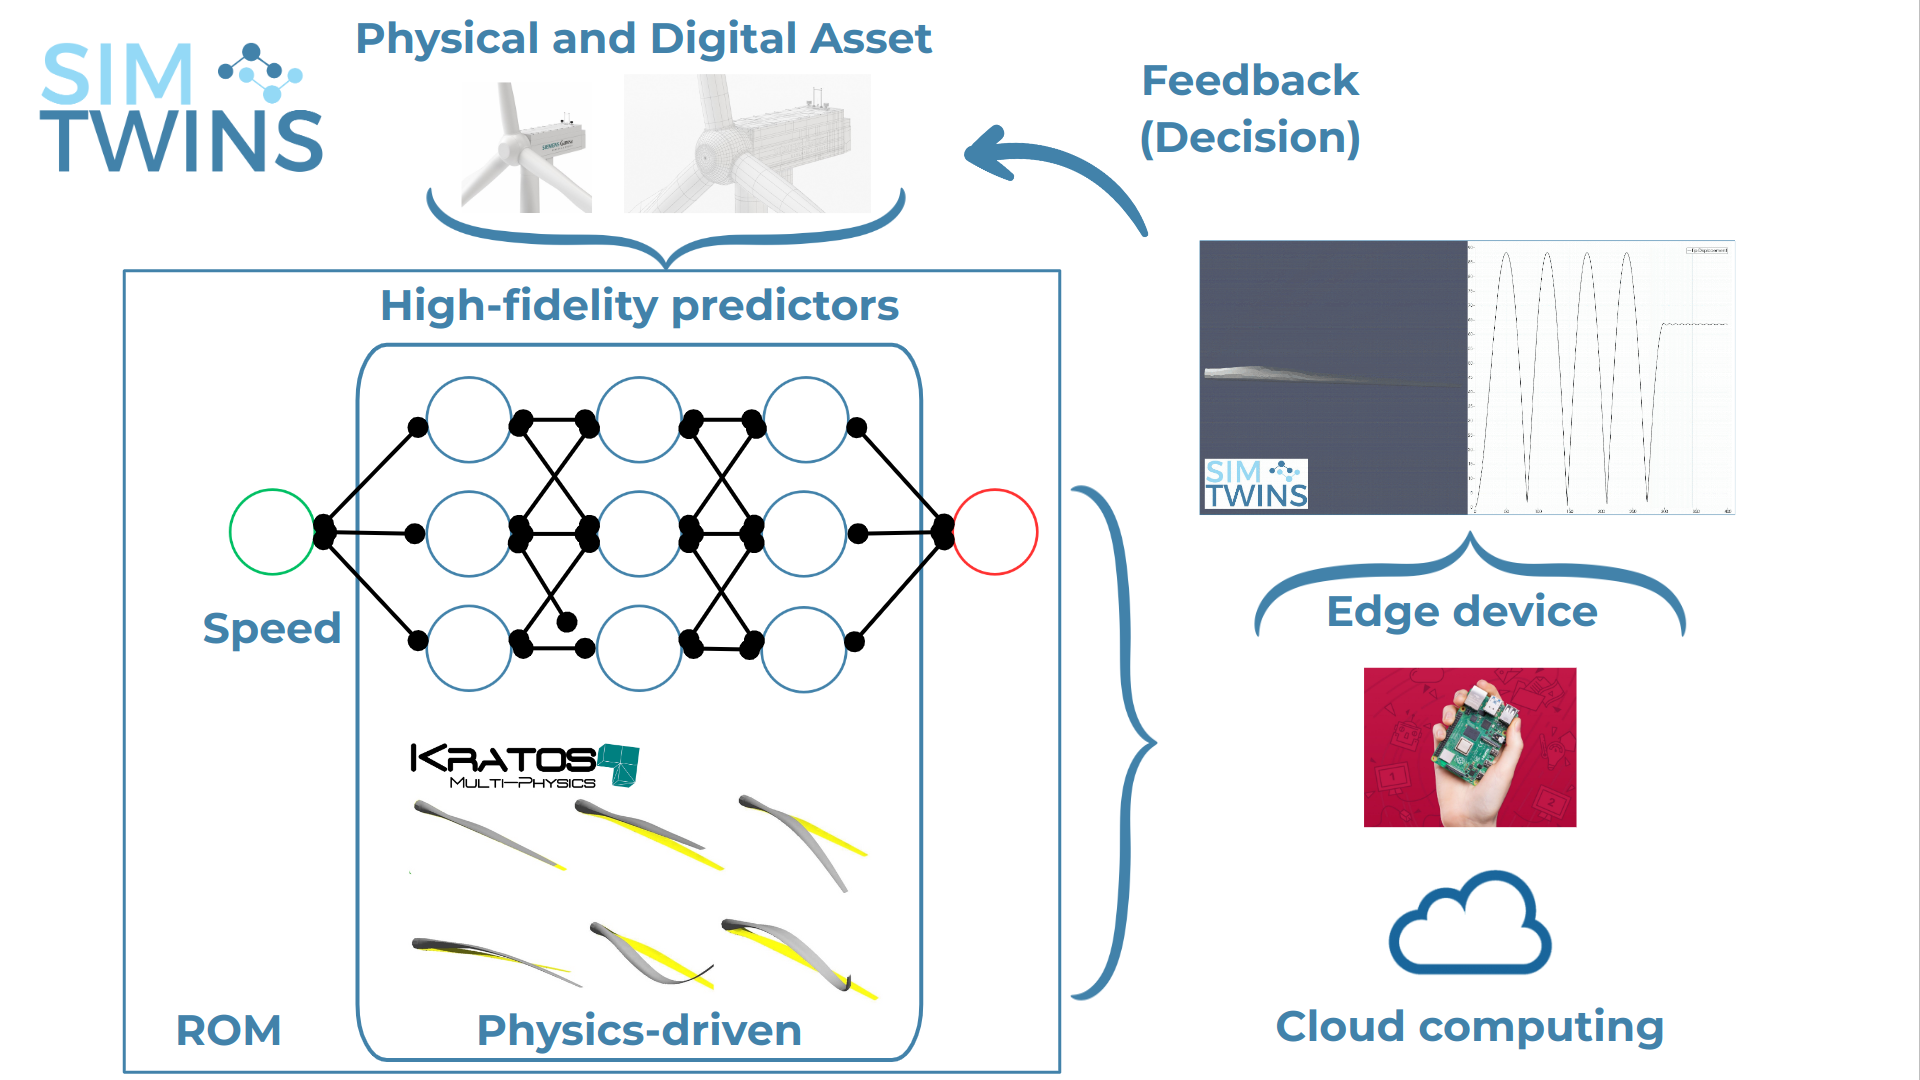
\includegraphics[trim=0mm 0mm 6mm 0mm, clip, width=0.92\textwidth]{Figures/DigitalTwinChartWindTurbine.png}
    \caption{Example of a wind turbine blade digital twin setup combining a physical asset, high-fidelity simulation-based predictors, and deployment across edge and cloud computing environments.}
    \label{fig:windturbine_digitaltwin}
\end{figure}

At the core of digital twins are simulation engines that replicate system behavior under varying conditions~\cite{hinchy2020using}. Despite their predictive power, high-fidelity simulations often demand substantial computational resources, constraining their practical application in scenarios that require rapid and repeated model evaluations. To address this challenge, ROMs have become integral components of digital twin technology. ROMs significantly reduce evaluation times and computational cost while preserving critical physical characteristics, enabling fast and accurate analyses required by digital twins~\cite{hartmann2018model, haas2012predictive}.

Among various ROM approaches, intrusive PROMs offer a compelling balance between accuracy, interpretability, and computational performance. Their preservation of the underlying physics and compatibility with advanced reduction methods make them especially suitable for digital twin applications in engineering. ROM-based digital twins are increasingly deployed via the \textit{Functional Mock-up Interface} (FMI) standard, which encapsulates ROMs into portable \textit{Functional Mock-up Units} (FMUs)~~\cite{blochwitz2011functional}. This approach enables seamless integration across diverse platforms and facilitates real-time interactions between simulations and operational systems. In this thesis, these concepts are consolidated into a parallel, scalable workflow designed explicitly for deploying ROM-based digital twins through FMUs in high-dimensional industrial scenarios~~\cite{Ares2024}.

Building upon these ideas, the present thesis proposes methodological advancements and robust implementation frameworks aimed at overcoming current limitations in ROM technologies. The subsequent sections formalize these motivations, outlining the specific research objectives and methodological approaches guiding this work.

\section{Approach and objectives}

To address the persistent gap between high-fidelity simulation capabilities and the real-time, scalable demands of modern digital twin applications, this thesis develops a cohesive framework for PROM that bridges the spectrum from simplified model problems to complex industrial scenarios. Recognizing that convection-dominated regimes, nonlinear dynamics, and extensive parametric studies pose significant challenges for conventional ROMs, this work systematically combines methodological advances in projection, hyper-reduction, nonlinear manifold closure, and HPC-enabled workflows.

The approach begins with the inviscid one-dimensional Burgers' equation, serving as a canonical model problem that clearly exposes the limitations of linear subspace approximations and motivates robust enhancements such as Petrov–Galerkin projection and residual-minimizing formulations. These insights are then scaled to more realistic engineering configurations, including the thermal dynamics of an electric motor within the eFlows4HPC context and the turbulent wake flow of the Ahmed body, a benchmark relevant to automotive industry aerodynamics, using Kratos Multiphysics and AERO-F. By embedding these developments within open-source platforms and implementing distributed training and hyper-reduction strategies, this thesis advances the practical deployment of PROMs for high-dimensional, real-time applications.

The specific objectives of this thesis are therefore to:
\begin{enumerate}
    \item Develop and assess linear projection-based ROMs (Galerkin, LSPG) for convection-dominated systems, using both canonical model problems and representative industry-like cases to characterize their performance and inherent limitations.
    \item Formulate and implement a novel hyper-reduction strategy for Petrov–Galerkin PROMs, enabling element-wise acceleration compatible with finite element assembly in Kratos Multiphysics.
    \item Design and validate a parallel HPC workflow for the scalable training and deployment of intrusive ROMs, demonstrated through an industrial digital twin application for motor thermal management within the eFlows4HPC framework.
    \item Advance physics consistency in neural-network-based manifolds through discrete physics-informed training strategies that align data-driven approximations with the residual behavior of the underlying numerical scheme.
    \item Extend the PROM methodology to nonlinear regimes by investigating latent-space closure strategies, including PROM-ANN and interpretable kernel-based surrogates (PROM-GPR, PROM-RBF), to mitigate the Kolmogorov $n$-width barrier, demonstrated on both model problems and more complex configurations such as the Ahmed body wake flow using AERO-F.
\end{enumerate}

Collectively, these objectives consolidate the thesis contributions toward robust, scalable, and physically consistent projection-based ROMs, enabling their practical use in high-dimensional, real-time digital twin applications for industrial contexts.

% \clearpage

% \section*{Nomenclature}

% \begin{tabular}{ll}
% HPC           & High-Performance Computing \\
% ROM           & Reduced Order Model \\
% PROM          & Projection-Based Reduced Order Model \\
% FOM           & Full Order Model \\
% POD           & Proper Orthogonal Decomposition \\
% RB            & Reduced Basis \\
% PGD           & Proper Generalized Decomposition \\
% PDE           & Partial Differential Equation \\
% FEM           & Finite Element Method \\
% SVD           & Singular Value Decomposition \\
% LSPG          & Least-Squares Petrov--Galerkin \\
% EIM           & Empirical Interpolation Method \\
% DEIM          & Discrete Empirical Interpolation Method \\
% GNAT          & Gauss--Newton with Approximated Tensors \\
% ECSW          & Energy-Conserving Sampling and Weighting \\
% ECM           & Empirical Cubature Method \\
% ANN           & Artificial Neural Network \\
% PINN          & Physics-Informed Neural Network \\
% DT            & Digital Twin \\
% FMU           & Functional Mock-up Unit \\
% FMI           & Functional Mock-up Interface \\
% UQ            & Uncertainty Quantification \\
% nn           & Number of retained POD modes \\
% nn-width     & Kolmogorov nn-width \\
% \end{tabular}
